% Created 2020-05-24 Sun 19:40
% Intended LaTeX compiler: pdflatex
\documentclass[10pt, compress, aspectratio=169, xcolor={table,usenames,dvipsnames}]{beamer}

\usepackage{booktabs}
\mode<beamer>{\usetheme[numbering=fraction, progressbar=none, titleformat=smallcaps, sectionpage=none]{metropolis}}
\usepackage{sourcecodepro}
\usepackage{booktabs}
\usepackage{array}
\usepackage{listings}
\usepackage{multirow}
\usepackage{caption}
\usepackage{xeCJK}
\usepackage{graphicx}
\usepackage[english]{babel}
\usepackage[scale=2]{ccicons}
\usepackage{hyperref}
\usepackage{relsize}
\usepackage{amsmath}
\usepackage{bm}
\usepackage{wasysym}
\usepackage{ragged2e}
\usepackage{textcomp}
\usepackage{pgfplots}
\usepgfplotslibrary{dateplot}
\definecolor{Base}{HTML}{191F26}
\definecolor{Accent}{HTML}{bb0300}
\setbeamercolor{alerted text}{fg=Accent}
\setbeamercolor{frametitle}{fg=Base,bg=White}
\setbeamercolor{normal text}{bg=black!2,fg=Base}
\setsansfont[BoldFont={Source Sans Pro Semibold},Numbers={OldStyle}]{Source Sans Pro}
\lstdefinelanguage{Julia}%
{morekeywords={abstract,struct,break,case,catch,const,continue,do,else,elseif,%
end,export,false,for,function,immutable,mutable,using,import,importall,if,in,%
macro,module,quote,return,switch,true,try,catch,type,typealias,%
while,<:,+,-,::,/},%
sensitive=true,%
alsoother={$},%
morecomment=[l]\#,%
morecomment=[n]{\#=}{=\#},%
morestring=[s]{"}{"},%
morestring=[m]{'}{'},%
}[keywords,comments,strings]%
\lstdefinelanguage{dockerfile}{
keywords={FROM, RUN, COPY, ADD, ENTRYPOINT, CMD,  ENV, ARG, WORKDIR, EXPOSE, LABEL, USER, VOLUME, STOPSIGNAL, ONBUILD, MAINTAINER},
sensitive=false,
comment=[l]{\#},
morestring=[b]',
morestring=[b]"
}
\lstdefinelanguage{yaml}{
keywords={true,false,null,y,n},
ndkeywords={},
sensitive=false,
comment=[l]{\#},
morecomment=[s]{/*}{*/},
morestring=[b]',
morestring=[b]"
}
\lstset{ %
backgroundcolor={},
basicstyle=\ttfamily\scriptsize,
breakatwhitespace=true,
breaklines=true,
captionpos=n,
commentstyle=\color{Accent},
extendedchars=true,
frame=n,
keywordstyle=\color{Accent},
rulecolor=\color{black},
showspaces=false,
showstringspaces=false,
showtabs=false,
stepnumber=2,
stringstyle=\color{gray},
tabsize=2,
}
\renewcommand*{\UrlFont}{\ttfamily\smaller\relax}
\graphicspath{{../../img/}}
\addtobeamertemplate{block begin}{}{\justifying}
\captionsetup[figure]{labelformat=empty}
\usetheme{default}
\author{ \vspace{-2em} \footnotesize Pedro Bruel \newline \scriptsize \emph{phrb@ime.usp.br}}
\date{\scriptsize May 25th, 2020}
\title{ Introduction to OS-Level Virtualization on Linux}
\hypersetup{
 pdfauthor={ \vspace{-2em} \footnotesize Pedro Bruel \newline \scriptsize \emph{phrb@ime.usp.br}},
 pdftitle={ Introduction to OS-Level Virtualization on Linux},
 pdfkeywords={},
 pdfsubject={},
 pdfcreator={Emacs 26.3 (Org mode 9.2.5)},
 pdflang={English}}
\begin{document}

\maketitle

\section{Introduction}
\label{sec:org5d1acfd}
\begin{frame}[label={sec:orge91a09b}]{What are Simulation, Emulation, Virtualization?}
\begin{columns}
\begin{column}{0.75\columnwidth}
\only<1-2>{
\begin{center}
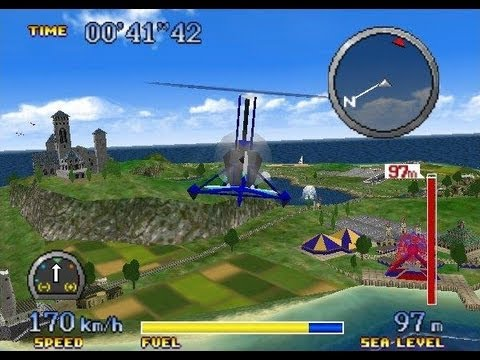
\includegraphics[width=0.7\columnwidth]{../../img/pilotwings64.jpg}
\end{center}
}
\only<3>{
\begin{center}
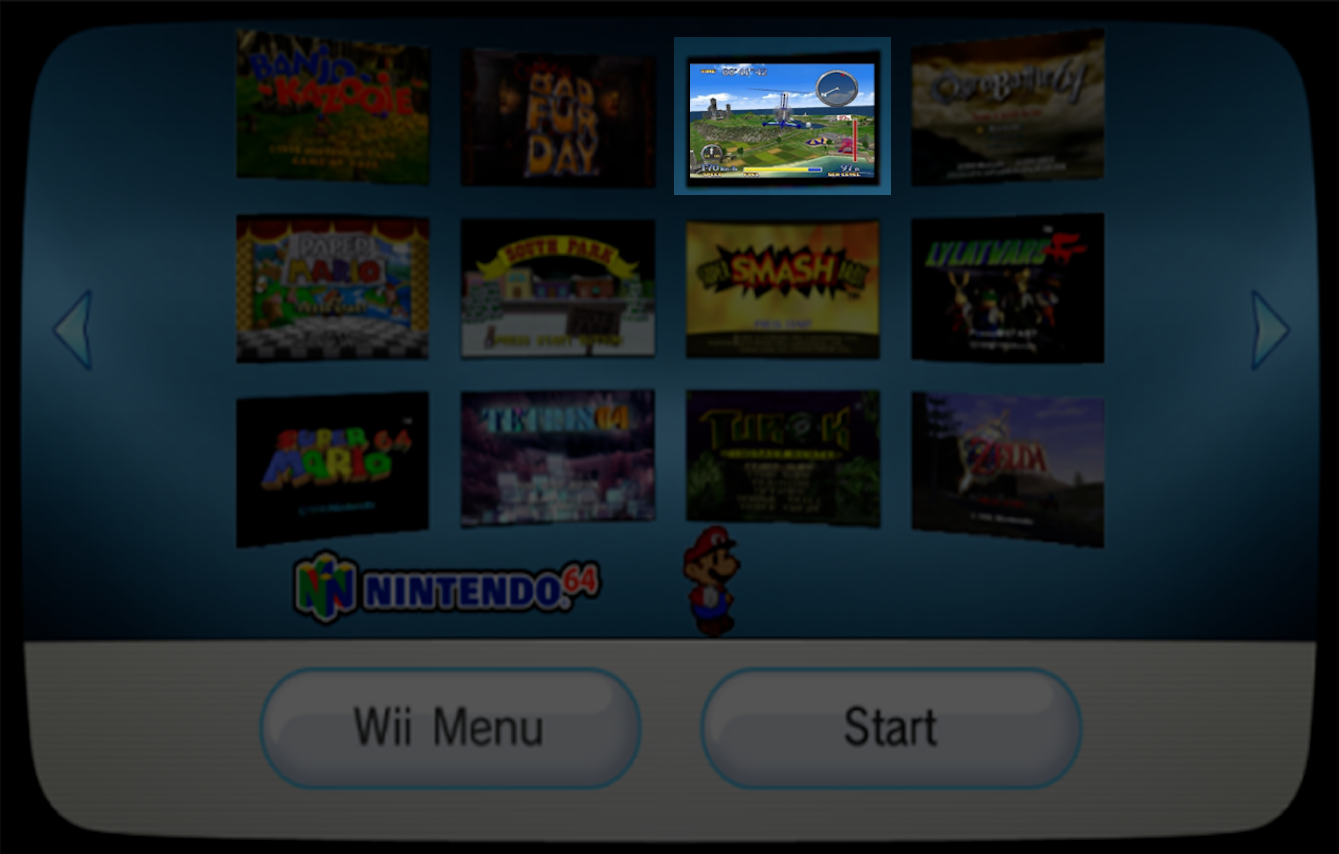
\includegraphics[width=0.9\columnwidth]{../../img/wii_n64.png}
\end{center}
}
\only<4>{
\begin{center}
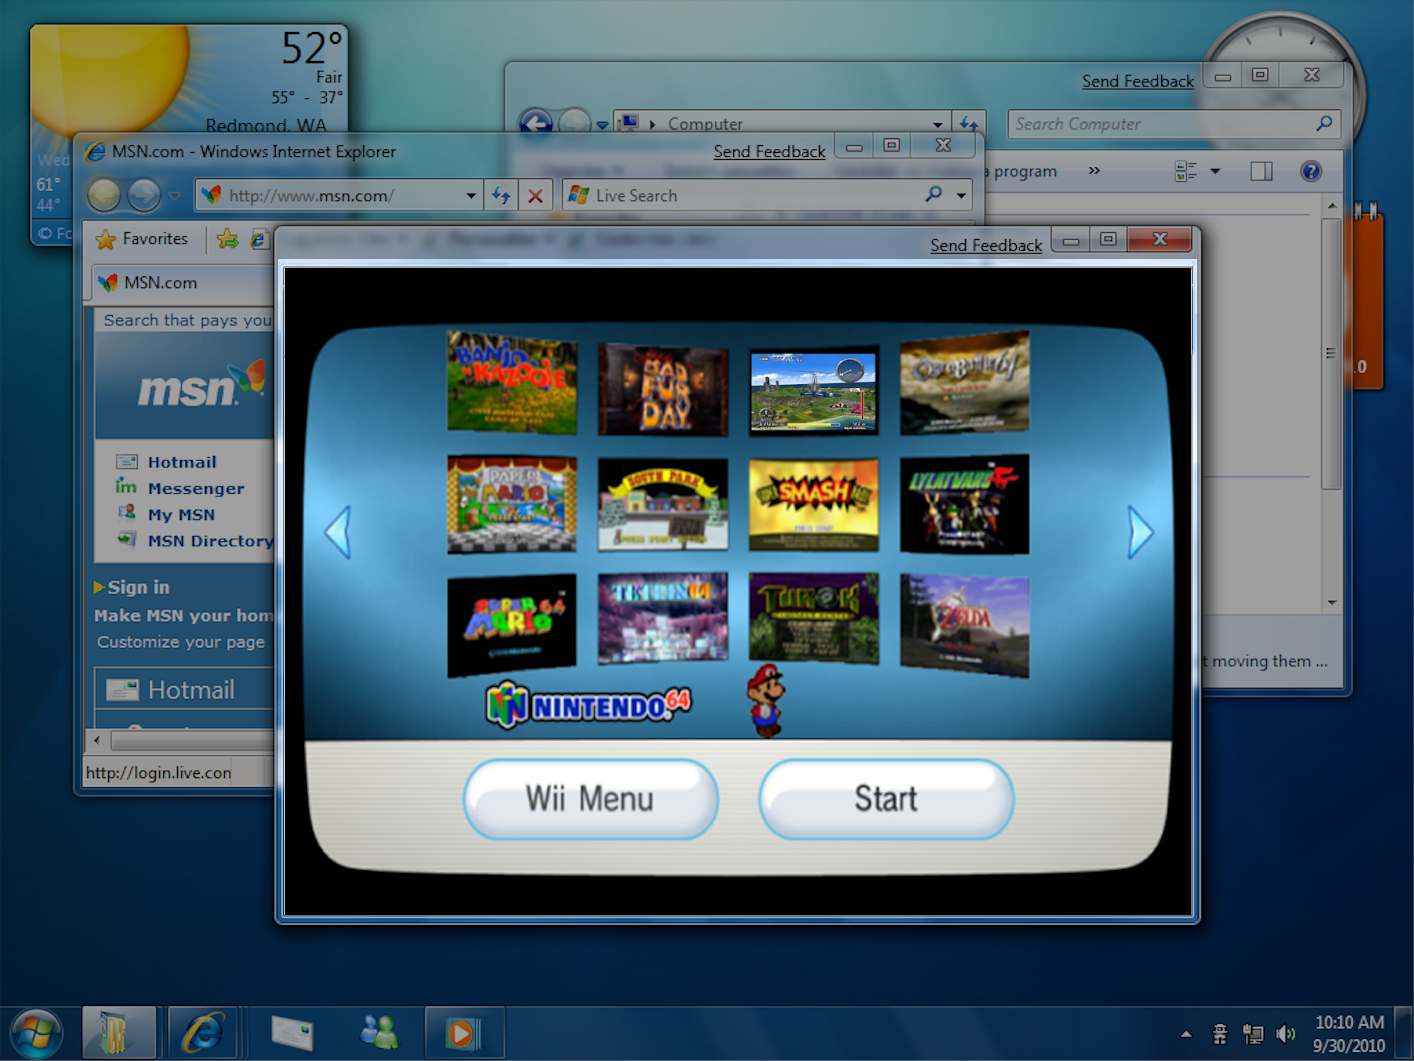
\includegraphics[width=0.9\columnwidth]{../../img/wii_n64_win7.png}
\end{center}
}
\only<5-6>{
\begin{center}
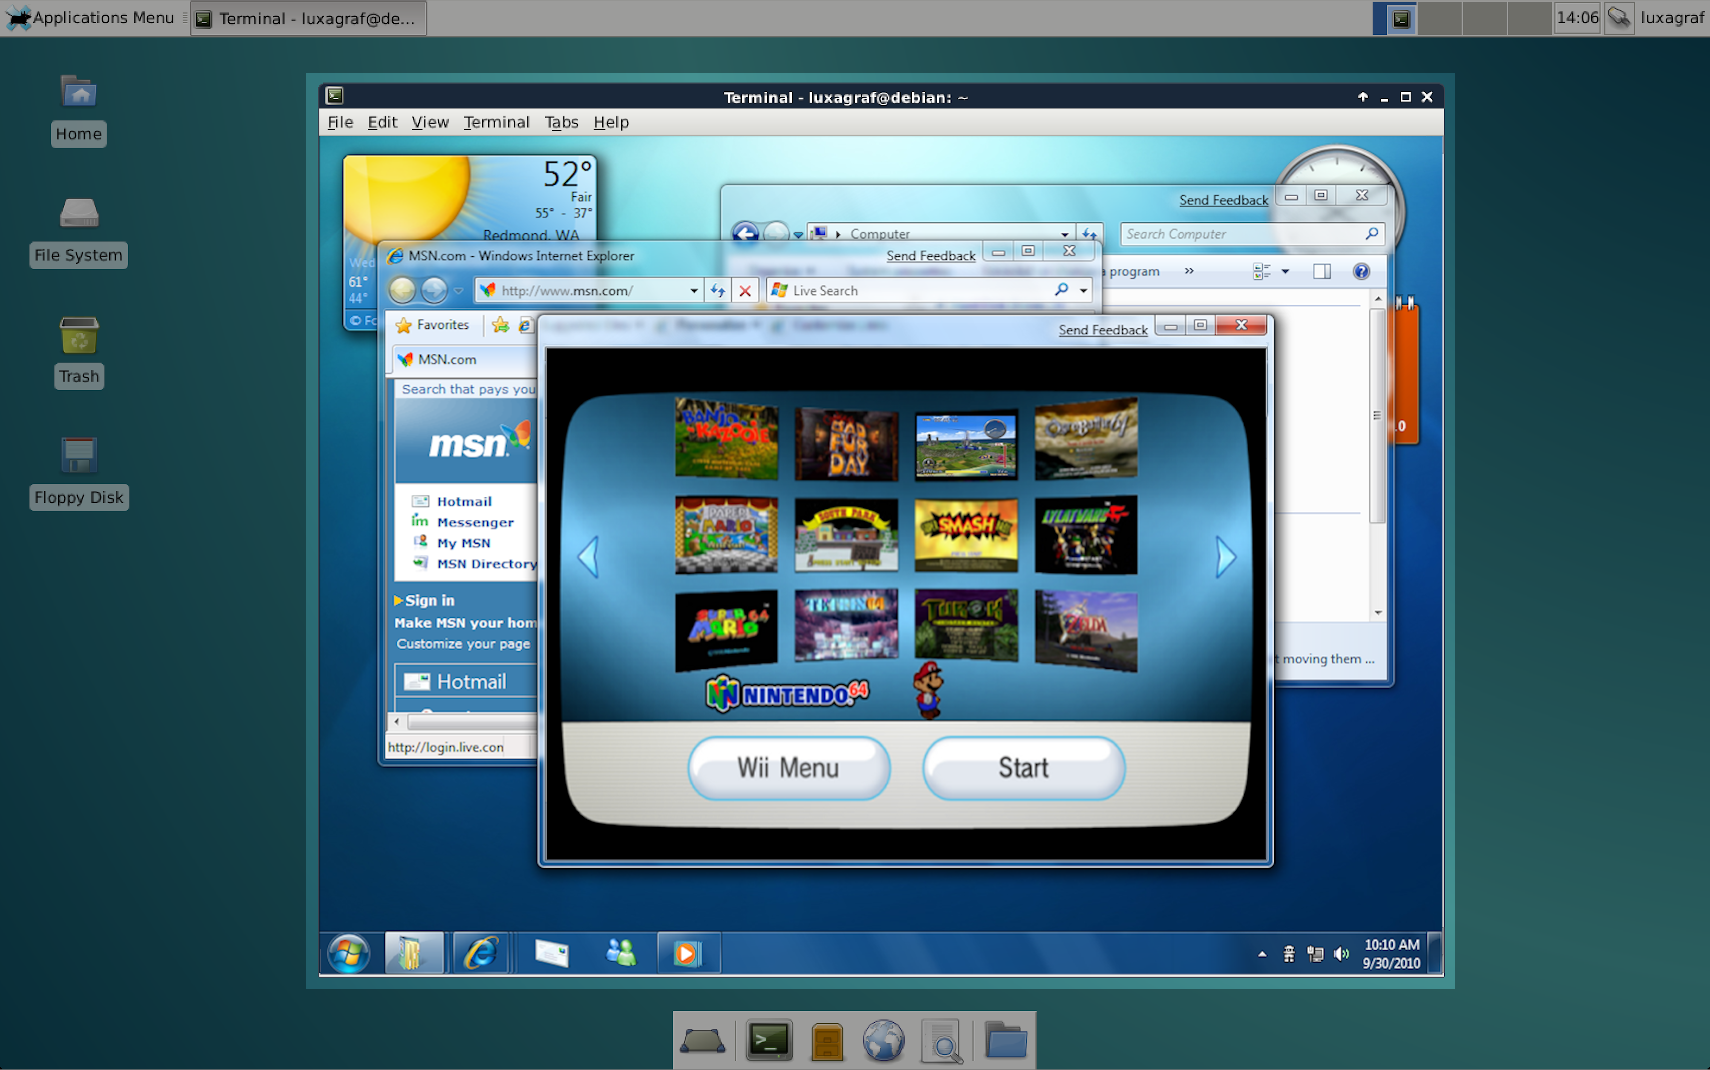
\includegraphics[width=0.9\columnwidth]{../../img/wii_n64_win7_debian.png}
\end{center}
}
\end{column}

\begin{column}{0.25\columnwidth}
\only<1>{
\begin{center}
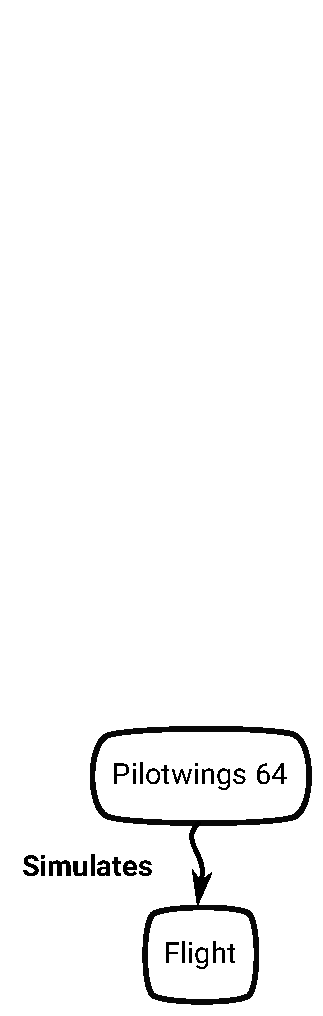
\includegraphics[width=.7\columnwidth]{../../img/pw64_flight.pdf}
\end{center}
}
\only<2>{
\begin{center}
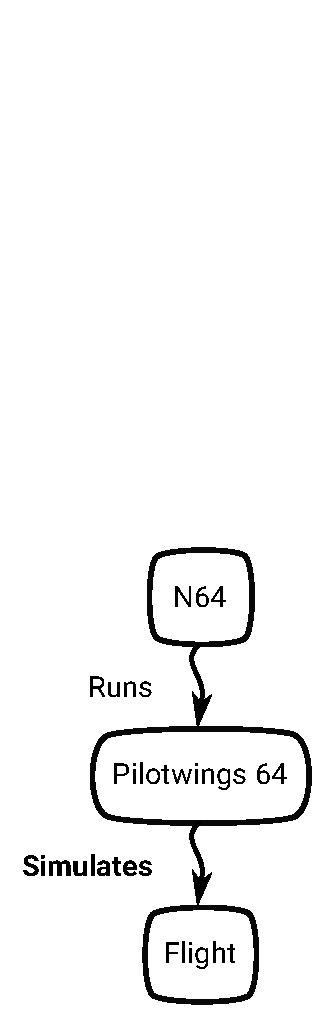
\includegraphics[width=.7\columnwidth]{../../img/n64_pw64_flight.pdf}
\end{center}
}
\only<3>{
\begin{center}
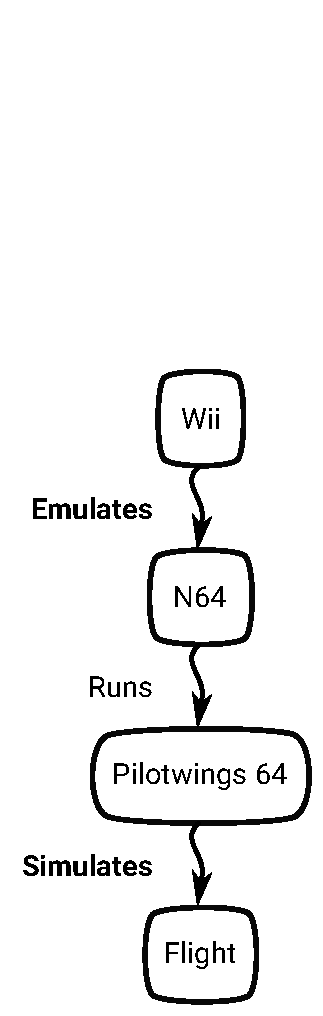
\includegraphics[width=.7\columnwidth]{../../img/wii_n64_pw64_flight.pdf}
\end{center}
}
\only<4>{
\begin{center}
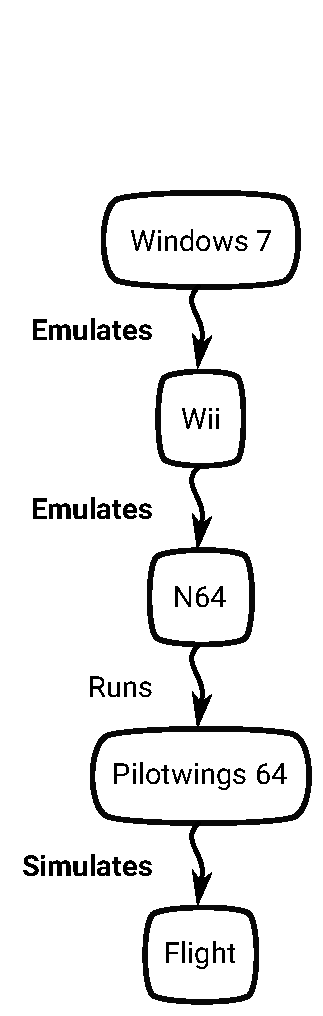
\includegraphics[width=.7\columnwidth]{../../img/win7_wii_n64_pw64_flight.pdf}
\end{center}
}
\only<5>{
\begin{center}
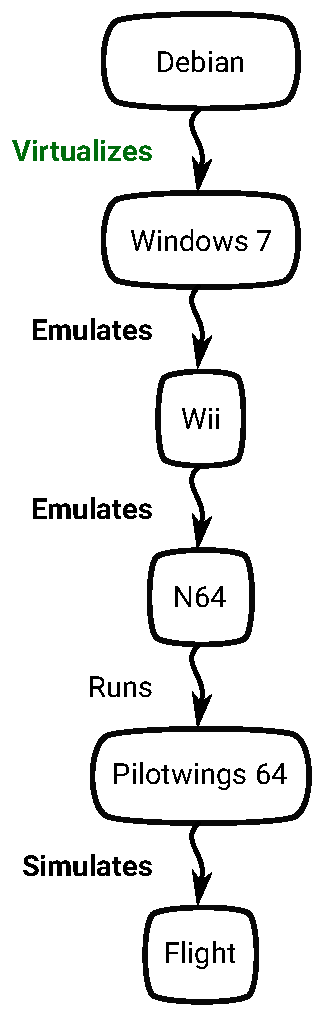
\includegraphics[width=.7\columnwidth]{../../img/debian_win7_wii_n64_pw64_flight.pdf}
\end{center}
}
\only<6>{
\begin{center}
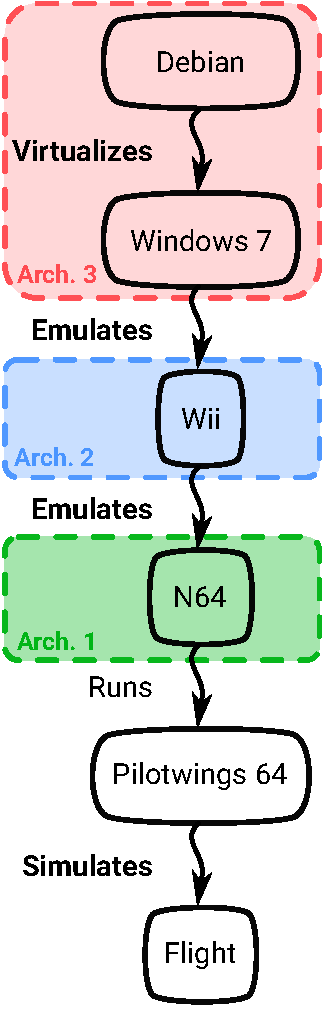
\includegraphics[width=.7\columnwidth]{../../img/arch_debian_win7_wii_n64_pw64_flight.pdf}
\end{center}
}
\end{column}
\end{columns}
\end{frame}
\begin{frame}[label={sec:org9ad4e7a}]{OS-Level Virtualization}
\begin{center}
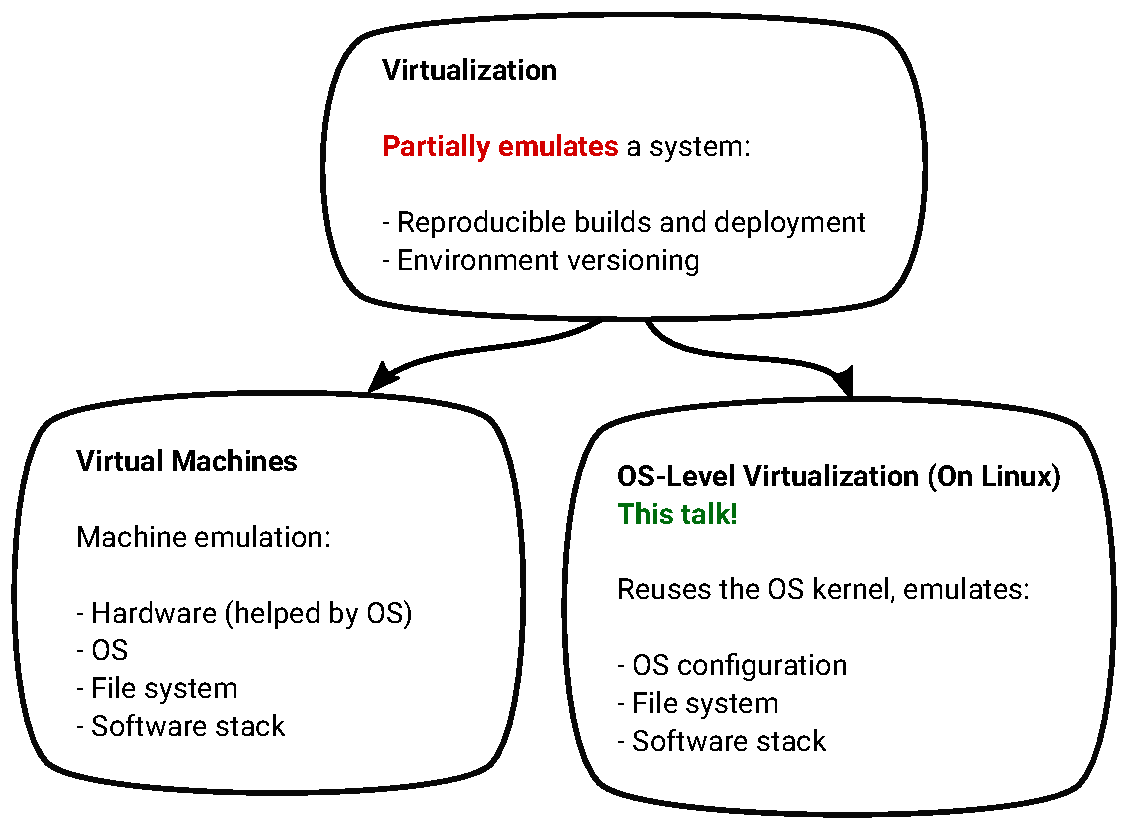
\includegraphics[width=.7\columnwidth]{../../img/virtualization_concept.pdf}
\end{center}
\end{frame}
\begin{frame}[label={sec:orge9dbc94}]{OS-Level Virtualization: Scope of this Talk}
\begin{columns}
\begin{column}{0.4\columnwidth}
\begin{block}{Scope}
\begin{itemize}
\item Why should you \alert{use containers}?
\begin{itemize}
\item Reproducible builds
\item Environment versioning
\item It's also \alert{easier}
\end{itemize}
\item How do containers \alert{work}?
\item What \alert{tools} are available?
\end{itemize}

\begin{center}

\includegraphics[width=.8\columnwidth]{../../img/containers.jpg}
\end{center}
\end{block}
\end{column}

\begin{column}{0.6\columnwidth}
\only<1>{
\begin{center}
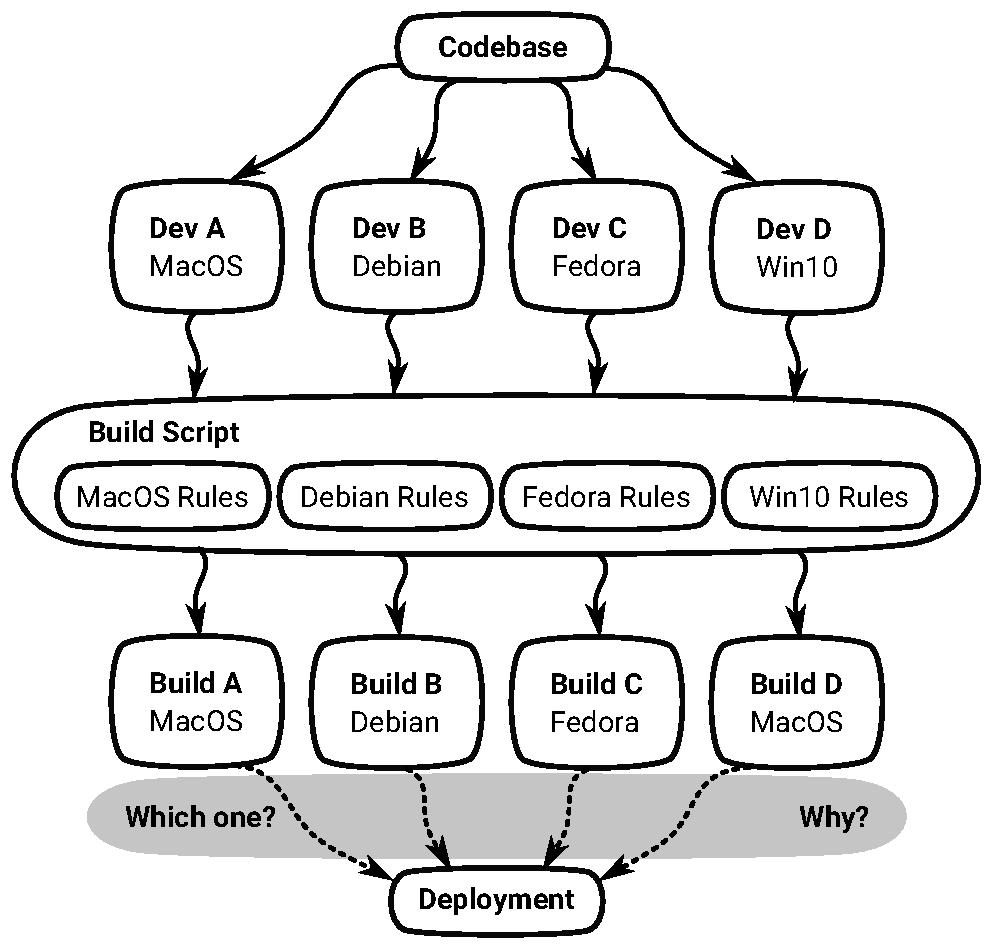
\includegraphics[width=.9\columnwidth]{../../img/project_no_containers.pdf}
\end{center}
}
\only<2>{
\begin{center}
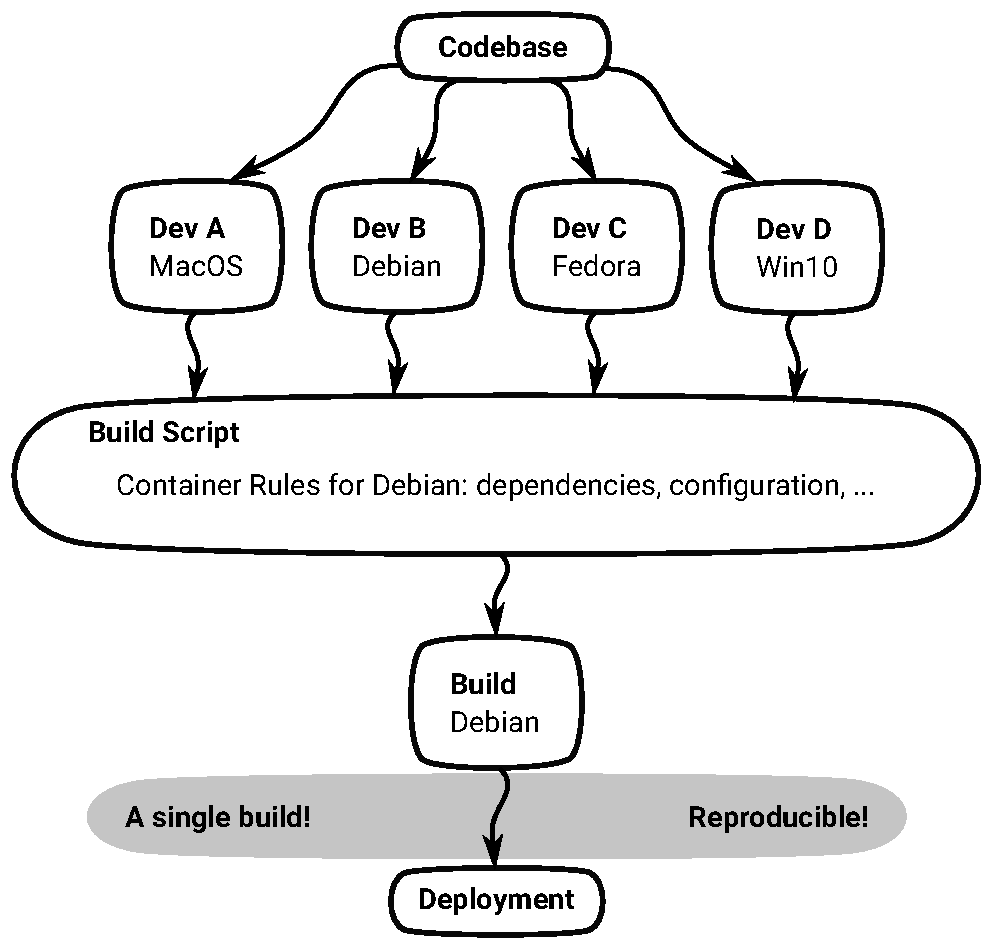
\includegraphics[width=.9\columnwidth]{../../img/project_with_containers.pdf}
\end{center}
}
\end{column}
\end{columns}
\end{frame}
\begin{frame}[label={sec:org914a470}]{OS-Level Virtualization on Linux}
\begin{center}
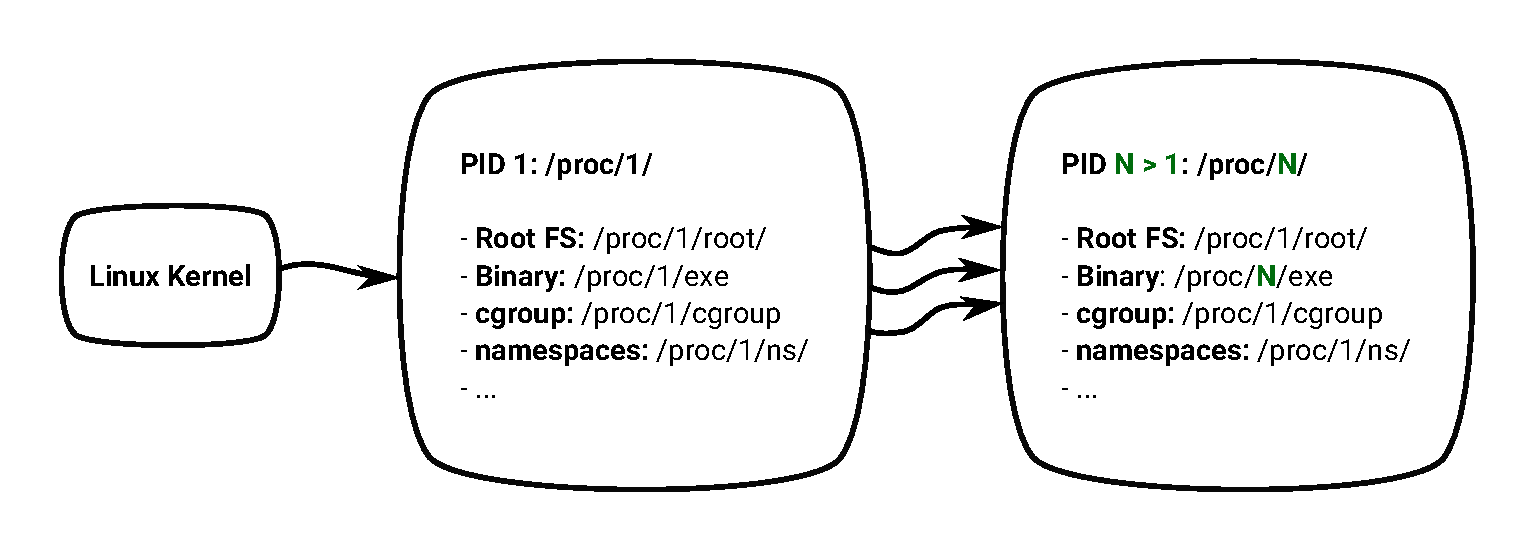
\includegraphics[width=\columnwidth]{../../img/virtualization_normal_kernel.pdf}
\end{center}
\end{frame}
\begin{frame}[label={sec:orgd5fb122}]{OS-Level Virtualization on Linux}
\begin{center}
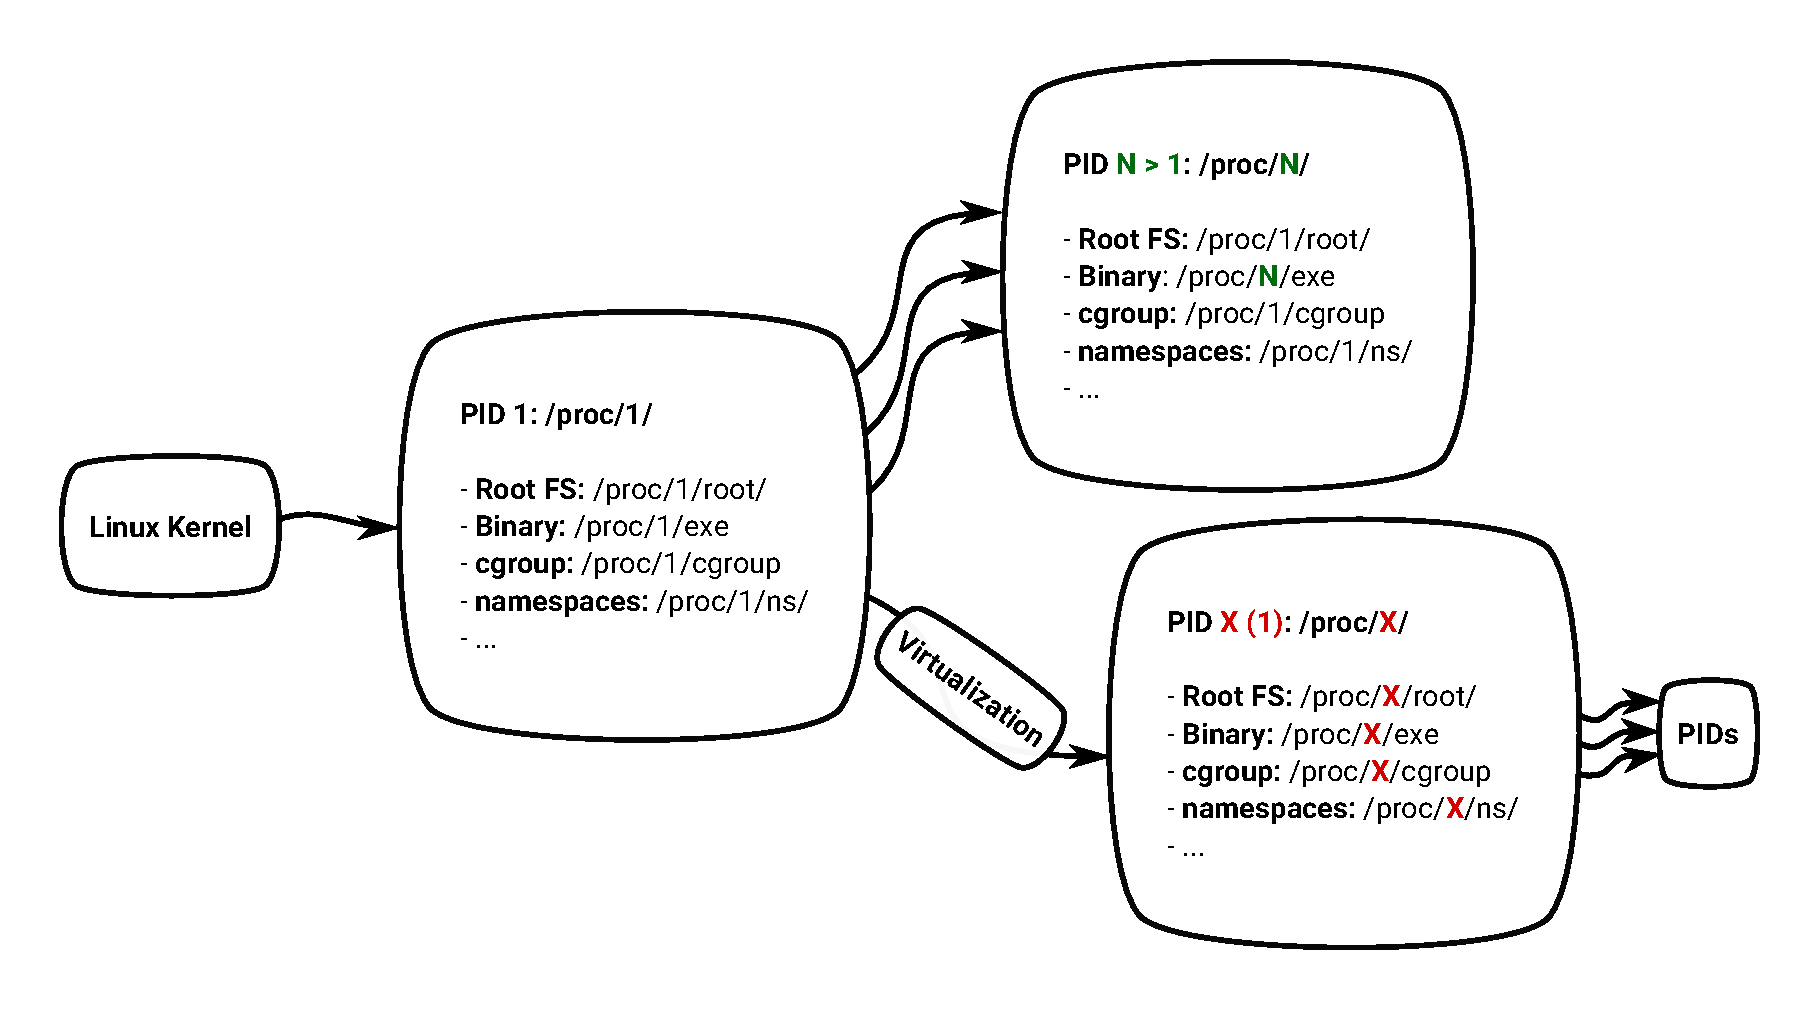
\includegraphics[width=\columnwidth]{../../img/virtualization_kernel.pdf}
\end{center}
\end{frame}
\section{Containers on Linux}
\label{sec:orgcb84d0b}
\begin{frame}[label={sec:org6b4a7a3}]{How do Containers Work?}
\begin{center}
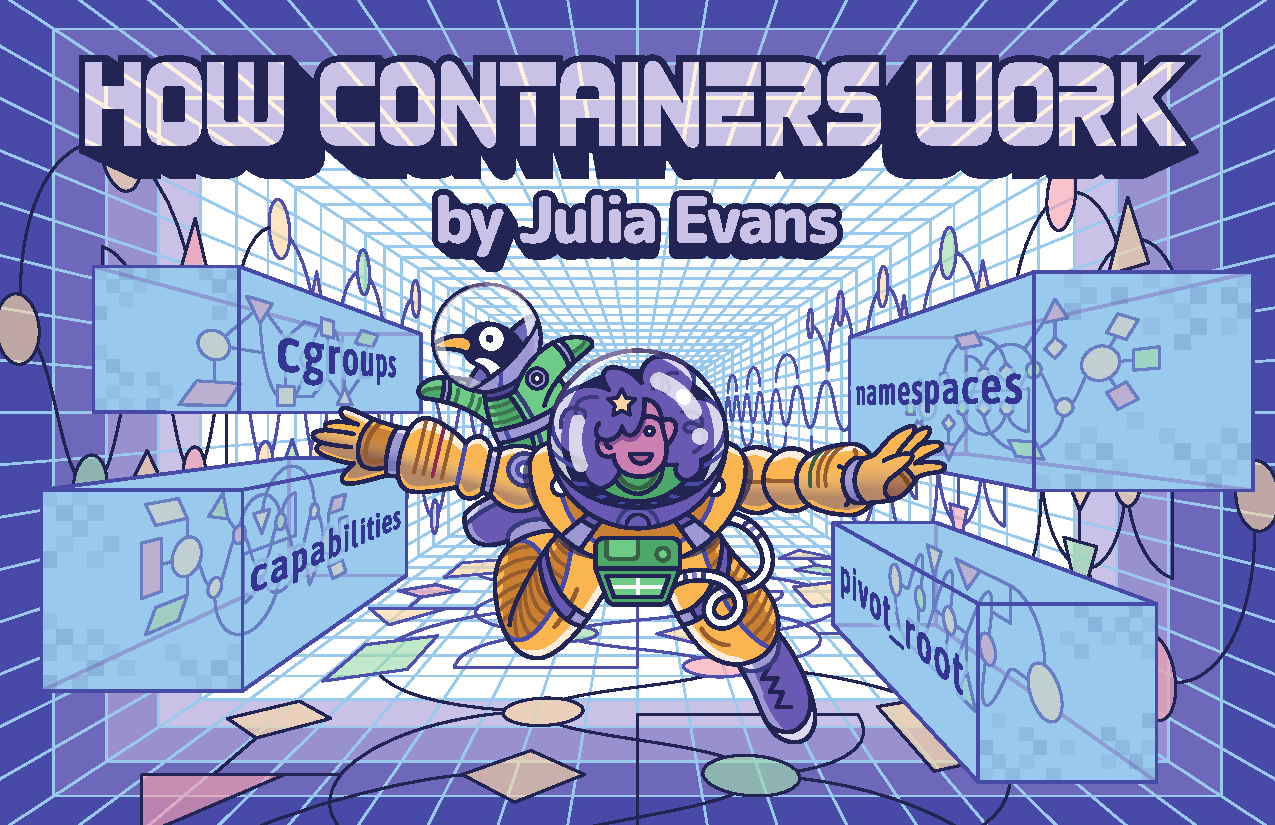
\includegraphics[width=.81\columnwidth]{../../img/how-containers-work_pg0.pdf}
\end{center}
\end{frame}
\begin{frame}[label={sec:org374af33}]{How do Containers Work?}
Images used \alert{with permission}:
\begin{center}
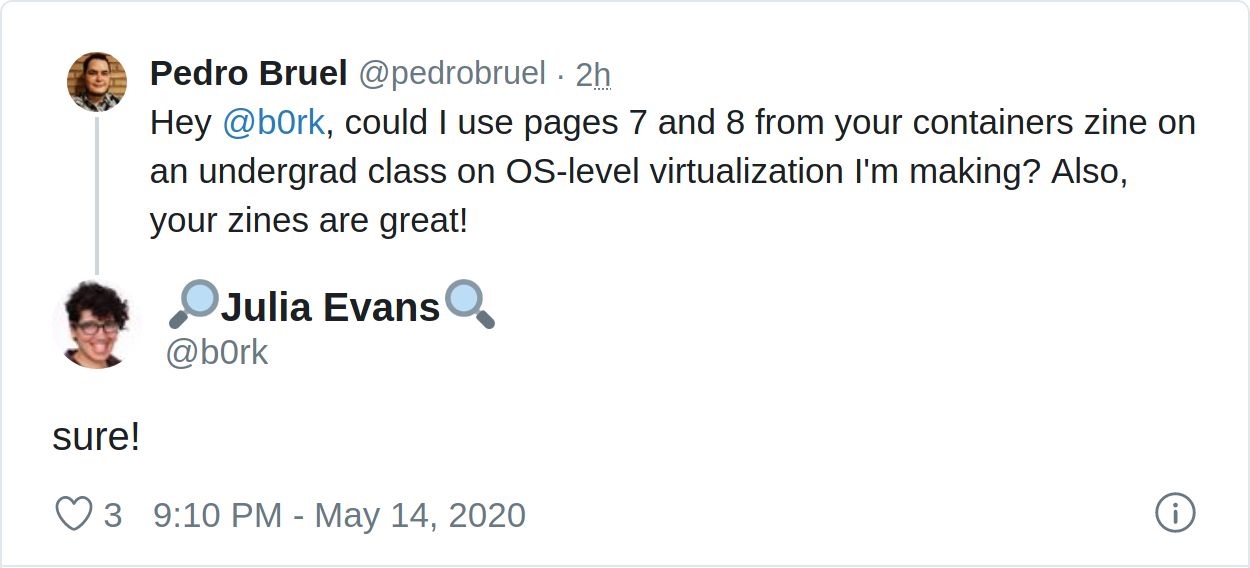
\includegraphics[width=.72\columnwidth]{../../img/hcw_permission_twitter.png}
\end{center}
\end{frame}
\begin{frame}[label={sec:orge191dc2}]{Containers on Linux are Just Processes}
\begin{center}
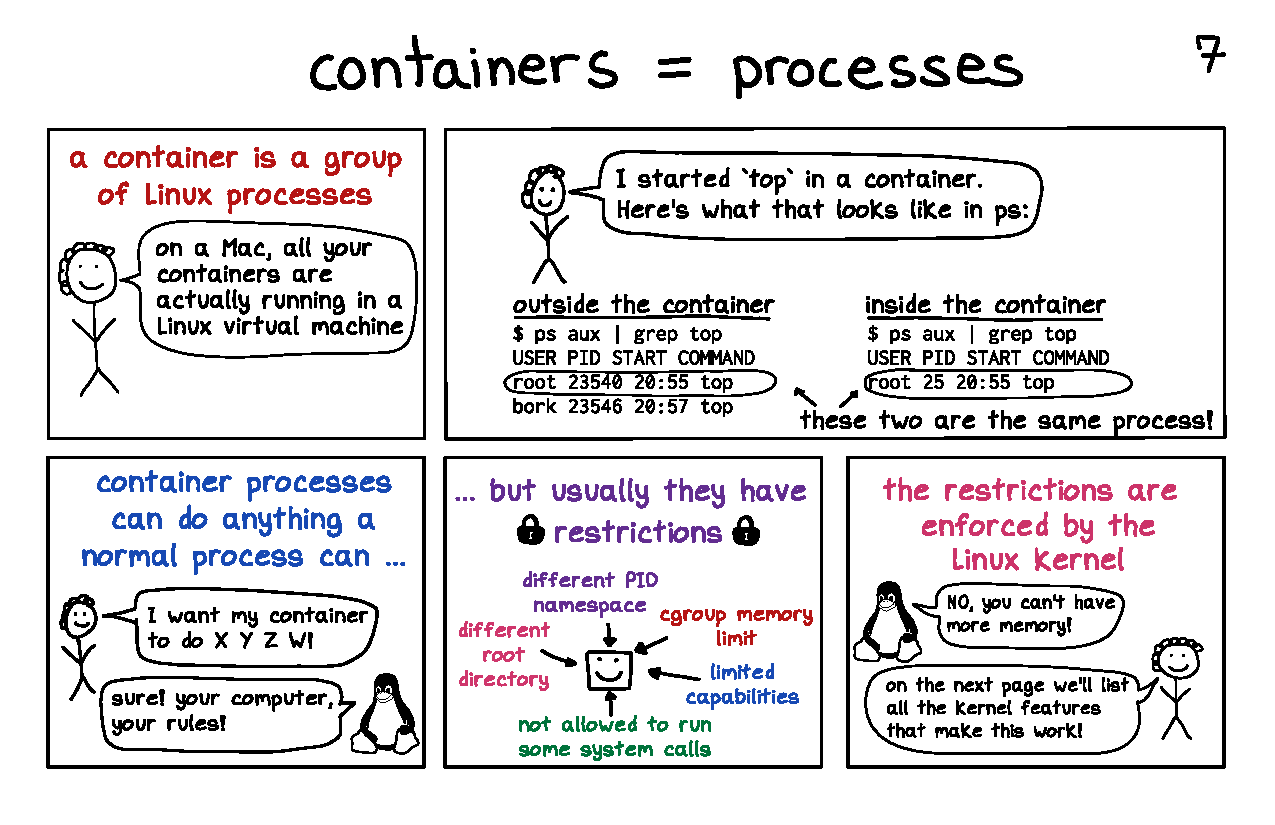
\includegraphics[width=.86\columnwidth]{../../img/how-containers-work_pg7.pdf}
\end{center}
\end{frame}
\begin{frame}[label={sec:org96b68ed}]{Containers on Linux use Some Kernel Features}
\begin{center}
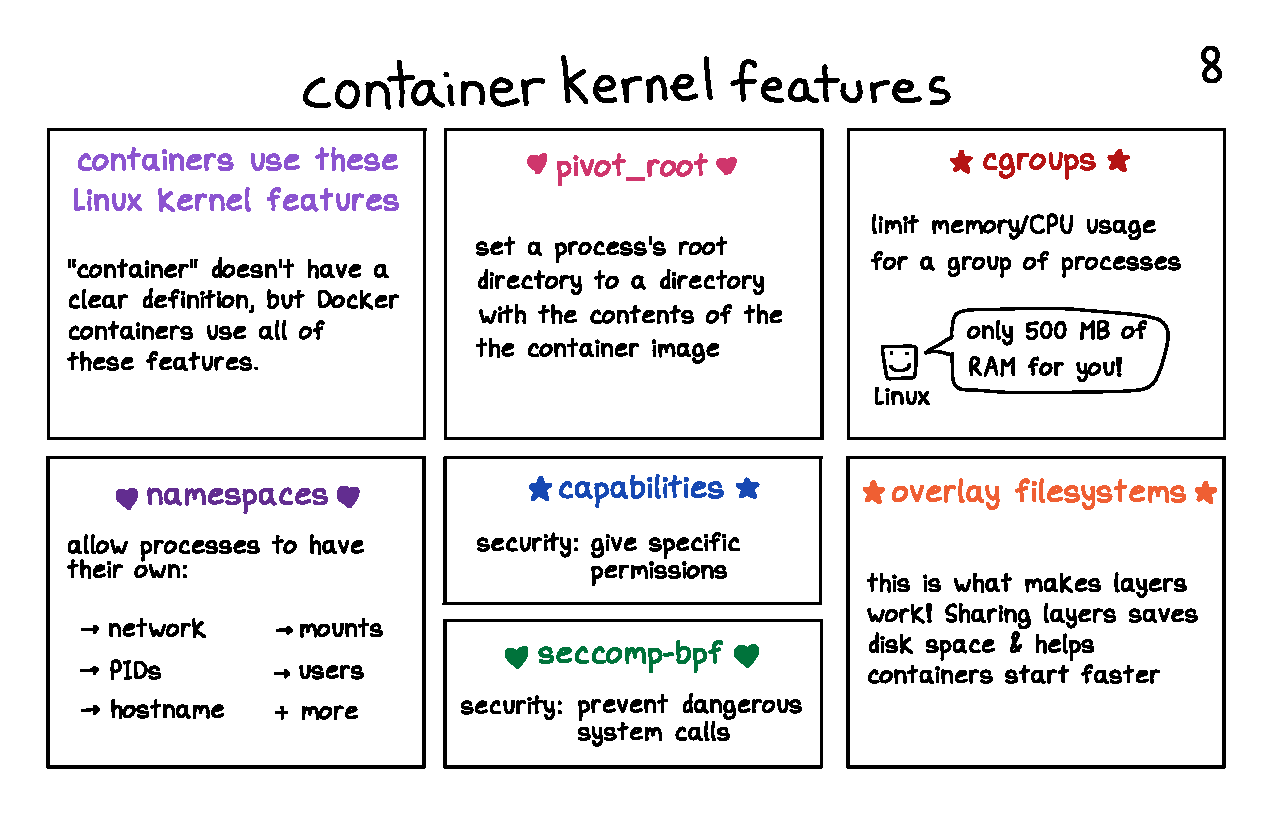
\includegraphics[width=.86\columnwidth]{../../img/how-containers-work_pg8.pdf}
\end{center}
\end{frame}
\section{Containers from Scratch}
\label{sec:orgdde33f8}
\begin{frame}[label={sec:org72b118f},fragile]{Containers from Scratch: Obtaing an Image}
 \begin{columns}
\begin{column}{0.5\columnwidth}
An \alert{image} usually means:

\begin{itemize}
\item A \alert{root} file system, and
\item Some \alert{metadata}
\end{itemize}
\end{column}
\begin{column}{0.5\columnwidth}
\begin{center}

\includegraphics[width=.5\columnwidth]{../../img/alpine_linux.png}
\end{center}

We will use the \alert{Alpine} distribution:
\begin{itemize}
\item It's root FS has only \alert{2.4MB}
\item No need for metadata
\end{itemize}
\end{column}
\end{columns}

\begin{block}{Bash Script}
\lstset{language=bash,label= ,caption= ,captionpos=b,numbers=none}
\begin{lstlisting}
#!/usr/bin/bash

IMG_DIR="alpine_img"
IMG_REPO="https://us.images.linuxcontainers.org/images"
IMG_URL="$IMG_REPO/alpine/3.11/amd64/default/20200521_13:00/rootfs.tar.xz"
[ ! -d $IMG_DIR ] && \
    mkdir -p $IMG_DIR && \
    curl $IMG_URL | tar xJ -C $IMG_DIR
\end{lstlisting}
\end{block}
\end{frame}

\begin{frame}[label={sec:org7470a36},fragile]{Containers from Scratch: Creating cgroups and Setting Limits}
 We will create a \alert{cgroup} allowing up to:
\begin{itemize}
\item \alert{50\%} CPU usage: 512/1024 \alert{shares}
\item \alert{10GB} of RAM
\end{itemize}

\begin{block}{Script}
\lstset{language=bash,label= ,caption= ,captionpos=b,numbers=none}
\begin{lstlisting}
CGROUP_ID="MAC0475-145"
sudo cgcreate -g "cpu,cpuacct,memory:$CGROUP_ID"
sudo cgset -r cpu.shares=512 "$CGROUP_ID"
sudo cgset -r memory.limit_in_bytes=10000000000 "$CGROUP_ID"
\end{lstlisting}
\end{block}
\end{frame}

\begin{frame}[label={sec:org8208c8f},fragile]{Containers from Scratch: Launching our Alpine Container}
 \begin{columns}
\begin{column}{0.5\columnwidth}
\begin{itemize}
\item \alert{cgexec}: Runs using a cgroup
\item \alert{unshare}: Runs with new \alert{namespaces}
\item \alert{chroot}: Changes \alert{root} of the file system
\end{itemize}
\end{column}
\begin{column}{0.5\columnwidth}
\begin{itemize}
\item \alert{mount}: Here, mounts a new \alert{proc} directory
\item \alert{sh}: Starts a shell on the \alert{container}
\item We could install \alert{depencies} now
\end{itemize}
\end{column}
\end{columns}

\begin{block}{Script}
\lstset{language=bash,label= ,caption= ,captionpos=b,numbers=none}
\begin{lstlisting}
HOSTNAME="alpine-container"
sudo cgexec -g "cpu,cpuacct,memory:$CGROUP_ID" \
     unshare -fmuipn --mount-proc \
     chroot "$IMG_DIR/" \
     /bin/sh -c "PATH=/bin && mount -t proc proc /proc && hostname $HOSTNAME && sh"

\end{lstlisting}

And some \alert{cleanup} after:

\lstset{language=bash,label= ,caption= ,captionpos=b,numbers=none}
\begin{lstlisting}
sudo cgdelete cpu,cpuacct,memory:/$CGROUP_ID
\end{lstlisting}
\end{block}
\end{frame}


\begin{frame}[label={sec:org3d6109f}]{Containers from Scratch: Resources}
\begin{columns}
\begin{column}{0.5\columnwidth}
\begin{block}{Talks}
\begin{itemize}
\item \href{https://www.youtube.com/watch?v=8fi7uSYlOdc}{Liz Rice, GOTO 2018}
\item \href{https://www.youtube.com/watch?v=\_TsSmSu57Zo}{Liz Rice, Container Camp}
\item \href{https://www.youtube.com/watch?v=I326bpbdvJo}{Antony Shaw, Pycon}
\end{itemize}
\begin{block}{Code}
\begin{itemize}
\item \href{https://github.com/lizrice/containers-from-scratch}{lizrice, containers from scratch in Go}
\item \href{https://github.com/p8952/bocker}{Bocker, docker in bash}
\item \href{https://github.com/tonybaloney/mocker}{Mocker, docker in python}
\end{itemize}
\end{block}
\end{block}
\end{column}
\begin{column}{0.5\columnwidth}
\begin{block}{Tutorials}
\begin{itemize}
\item \href{https://btholt.github.io/complete-intro-to-containers/}{btholt, Complete Intro to Containers}
\end{itemize}

\begin{center}

\includegraphics[width=.99\columnwidth]{../../img/lizrice_goto2018.jpg}
\end{center}
\end{block}
\end{column}
\end{columns}
\end{frame}
\section{Docker Containers}
\label{sec:orgf6be905}
\begin{frame}[label={sec:org1fd8058},fragile]{The Docker API for Containers}
 \only<1>{
\begin{center}
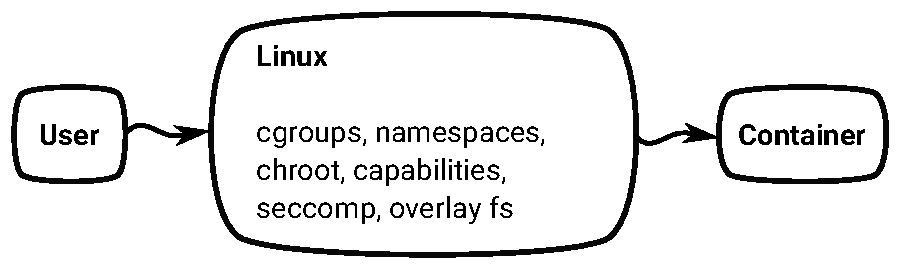
\includegraphics[width=.6\columnwidth]{../../img/virt_no_docker.pdf}
\end{center}
}
\only<2-3>{
\begin{center}
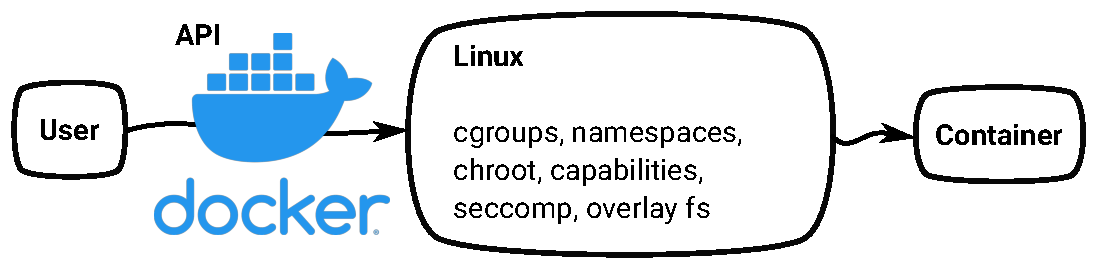
\includegraphics[width=.7\columnwidth]{../../img/virt_with_docker.pdf}
\end{center}
}

\begin{block}<3>{Reproducing the Alpine Container}
\lstset{language=bash,label= ,caption= ,captionpos=b,numbers=none}
\begin{lstlisting}
#! /bin/bash

sudo docker image pull alpine
sudo docker container run -it --memory=10g --cpu-shares=512 alpine
\end{lstlisting}
\end{block}
\end{frame}

\begin{frame}[label={sec:orgef5f792},fragile]{The Docker API for Containers}
 Some \alert{API functions}:
\footnotesize
\begin{center}
\begin{tabular}{p{0.1\columnwidth}p{0.1\columnwidth}p{0.06\columnwidth}p{0.22\columnwidth}p{0.28\columnwidth}}
\toprule
\textbf{Docker API} &  &  & \textbf{Description} & \textbf{In Our Script}\\
\midrule
 \multirow{9}{*}{\texttt{docker}} &  \multirow{4}{*}{\texttt{image}} & \texttt{pull} & Downloads images & \texttt{mkdir}, \texttt{curl}, \texttt{tar}\\
 &  & \texttt{ls} & Lists downloaded images & \\
 &  & \texttt{save} & Writes image to a \texttt{.tar} & \\
 &  & \texttt{build} & Builds an image & \\
 &  &  &  & \\
 &  \multirow{4}{*}{\texttt{container}} & \texttt{run} & Runs containers in images & \texttt{cgcreate}, \texttt{cgset}, \texttt{cgexec}, \texttt{unshare}, \texttt{chroot}, \texttt{hostname}, \texttt{mount}\\
 &  & \texttt{ls} & Lists running containers & \\
 &  & \texttt{attach} & Attaches to a container & \\
 &  & \texttt{commit} & Saves container to image & \\
\bottomrule
\end{tabular}
\end{center}
\normalsize
\begin{itemize}
\item Check the examples and \href{https://docs.docker.com/engine/reference/commandline/cli/}{the docs} for more
\end{itemize}
\end{frame}
\section{Dockerfiles}
\label{sec:orgd622b0d}
\begin{frame}[label={sec:orga1a85da}]{Environment Versioning with Dockerfiles}
\only<1>{
\begin{center}
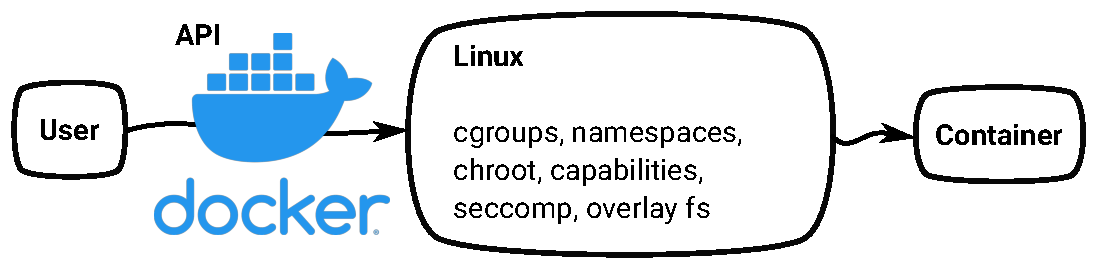
\includegraphics[width=.64\columnwidth]{../../img/virt_with_docker.pdf}
\end{center}
}
\only<2>{
\begin{center}
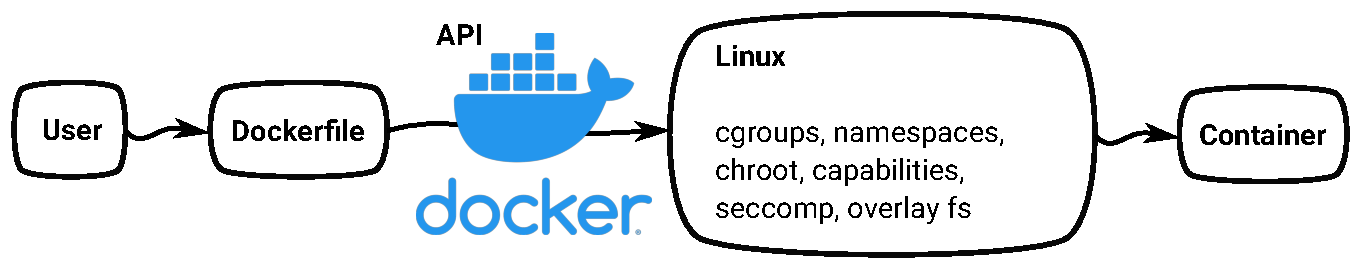
\includegraphics[width=.78\columnwidth]{../../img/virt_with_dockerfile.pdf}
\end{center}
}
\begin{block}{Dockerfiles}
\begin{itemize}
\item Similar to \alert{makefiles}
\item Define container \alert{properties}:
\begin{itemize}
\item Versions of images from \href{https://hub.docker.com/search?q=\&type=image}{dockerhub}
\item Environment variables
\item Install dependencies
\end{itemize}
\end{itemize}
\end{block}
\end{frame}
\begin{frame}[label={sec:org1147c79},fragile]{Dockerfiles: A Simple Bulletin Board}
 \begin{block}{Cloning the Repository}
\lstset{language=bash,label= ,caption= ,captionpos=b,numbers=none}
\begin{lstlisting}
git clone https://github.com/dockersamples/node-bulletin-board
\end{lstlisting}
\end{block}
\begin{block}{Dockerfile}
\lstset{language=dockerfile,label= ,caption= ,captionpos=b,numbers=none}
\begin{lstlisting}
FROM node:current-slim
WORKDIR /usr/src/app
COPY package.json .
RUN npm install
EXPOSE 8080
CMD [ "npm", "start" ]
COPY . .
\end{lstlisting}
\end{block}
\end{frame}
\begin{frame}[label={sec:orga8133bd},fragile]{Dockerfiles: Building and Running}
 \begin{block}{Building the Image}
\lstset{language=bash,label= ,caption= ,captionpos=b,numbers=none}
\begin{lstlisting}
cd node-bulletin-board/bulletin-board-app
sudo docker image build --tag bulletinboard:1.0 .
sudo docker container run --publish 8000:8080 --detach --name bb bulletinboard:1.0
\end{lstlisting}
\end{block}

\begin{block}{Cleaning up}
\lstset{language=bash,label= ,caption= ,captionpos=b,numbers=none}
\begin{lstlisting}
cd node-bulletin-board/bulletin-board-app
sudo docker container rm --force bb
\end{lstlisting}

\begin{itemize}
\item Check the \href{https://docs.docker.com/get-started/part2/}{complete tutorial}
\end{itemize}
\end{block}
\end{frame}
\section{Docker Compose}
\label{sec:orgca8e6ac}
\begin{frame}[label={sec:org7a9fe2e}]{Combining Services with Docker Compose}
\only<1>{
\begin{center}
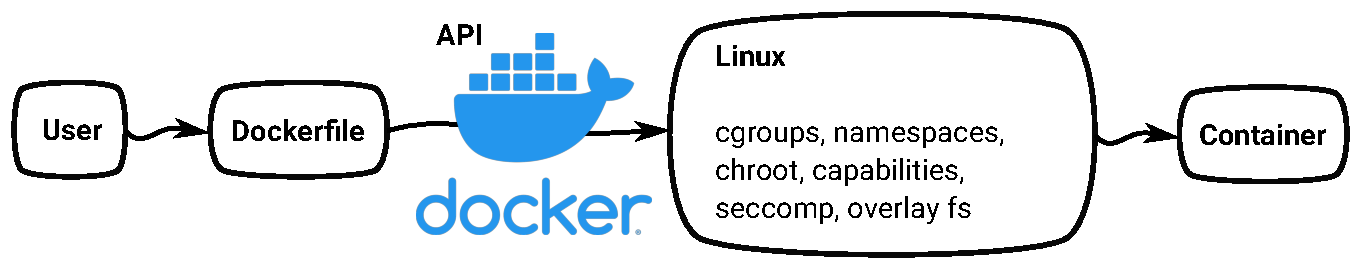
\includegraphics[width=.81\columnwidth]{../../img/virt_with_dockerfile.pdf}
\end{center}
}
\only<2>{
\begin{center}
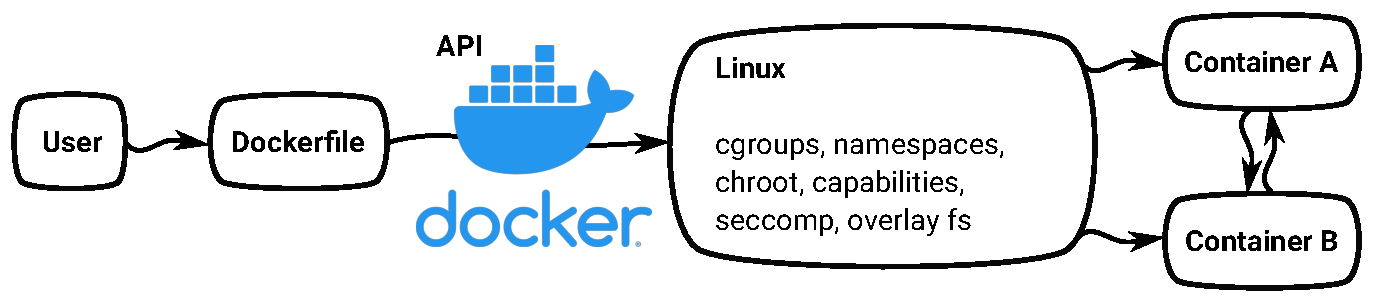
\includegraphics[width=.94\columnwidth]{../../img/virt_with_docker_compose.pdf}
\end{center}
}
\begin{block}{Docker-compose}
\begin{itemize}
\item Uses \alert{Dockerfiles} too
\item Defines \alert{services} on \alert{separate containers}:
\begin{itemize}
\item Configure service \alert{communication}
\item Maintain separate service \alert{projects}
\end{itemize}
\end{itemize}
\end{block}
\end{frame}
\begin{frame}[label={sec:orgd03b029},fragile]{Combining Services with Docker Compose: Flask + Redis}
 \lstset{language=Python,label= ,caption= ,captionpos=b,numbers=none}
\begin{lstlisting}
import time, redis
from flask import Flask

app = Flask(__name__)
cache = redis.Redis(host = 'redis', port = 6379)

def get_hit_count():
    retries = 5
    while True:
        try:
            return cache.incr('hits')
        except redis.exceptions.ConnectionError as exc:
            if retries == 0:
                raise exc
            retries -= 1
            time.sleep(0.5)

@app.route('/')
def hello():
    count = get_hit_count()
    return 'Hello World! I have been seen {} times.\n'.format(count)
\end{lstlisting}
\end{frame}

\begin{frame}[label={sec:org838e644},fragile]{Combining Services with Docker Compose: Flask + Redis}
 \begin{block}{Flask Dockerfile}
\begin{itemize}
\item Use an Alpine image, with Python 3.7
\item Configure and install \alert{Flask} dependencies
\item Define a default \alert{container command}
\end{itemize}

\lstset{language=dockerfile,label= ,caption= ,captionpos=b,numbers=none}
\begin{lstlisting}
FROM python:3.7-alpine
WORKDIR /code
ENV FLASK_APP app.py
ENV FLASK_RUN_HOST 0.0.0.0
RUN apk add --no-cache gcc musl-dev linux-headers
COPY requirements.txt requirements.txt
RUN pip install -r requirements.txt
COPY . .
CMD ["flask", "run"]
\end{lstlisting}
\end{block}
\end{frame}

\begin{frame}[label={sec:org4f461e1},fragile]{Combining Services with Docker Compose: Flask + Redis}
 \begin{block}{Docker Compose Configuration}
\begin{itemize}
\item Define \alert{service architecture}
\item Use the \alert{default} Redis Alpine image
\end{itemize}

\lstset{language=yaml,label= ,caption= ,captionpos=b,numbers=none}
\begin{lstlisting}
version: '3'
services:
  web:
    build: .
    ports:
      - "5000:5000"
    volumes:
      - .:/code
    environment:
      FLASK_ENV: development
  redis:
    image: "redis:alpine"
\end{lstlisting}

\begin{itemize}
\item Check the \href{https://docs.docker.com/compose/gettingstarted/}{complete tutorial}
\end{itemize}
\end{block}
\end{frame}
\section{Conclusion}
\label{sec:orgd9d8560}
\begin{frame}[label={sec:org2e2610f}]{OS-Level Virtualization: Conclusion}
\begin{columns}
\begin{column}{0.4\columnwidth}
\begin{block}{Take-away}
\begin{itemize}
\item You should \alert{use containers}!
\begin{itemize}
\item Reproducible builds
\item Environment versioning
\item It's \alert{easy}
\end{itemize}
\item Containers are \alert{processes}
\item Many \alert{tools} are available:
\end{itemize}

\begin{center}

\includegraphics[width=.8\columnwidth]{../../img/containers.jpg}
\end{center}
\end{block}
\end{column}

\begin{column}{0.6\columnwidth}
\only<1>{
\begin{center}
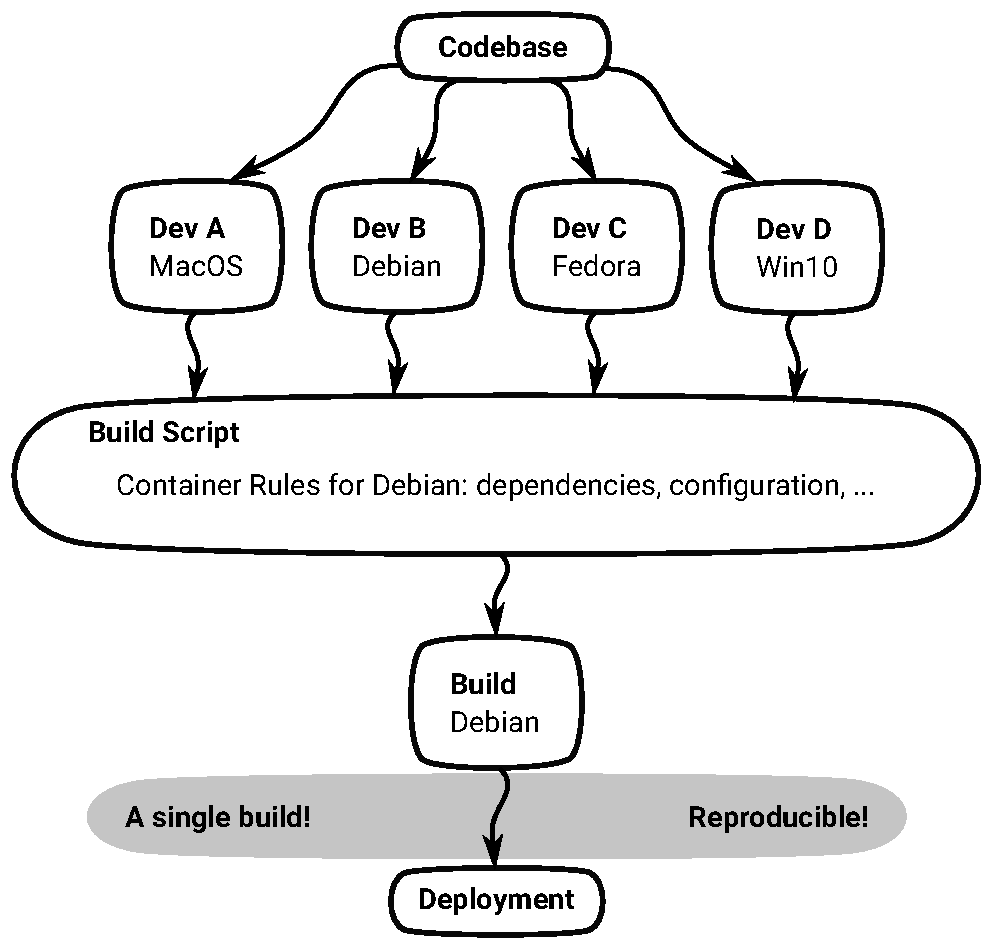
\includegraphics[width=.9\columnwidth]{../../img/project_with_containers.pdf}
\end{center}
}
\end{column}
\end{columns}
\end{frame}
\end{document}
